\section{Accepttest}
\label{forforstaerker_accepttest}

Kravene specifikt til forforstærkeren er opstillet i tabel \ref{tab:krav_forforstaerker} og med henblik på at teste dem, er der udført målinger som beskrevet i Appendiks D??. Indgangsimpedansen er, som vist i tabel \ref{tab:resultatimpedans_forforstaerker}, med målingerne beregnet til 22,1 k\ohm~. Kravet lyder på 22 k\ohm, hvilket dermed ikke umiddelbart er opnået. Dog kan tolerancen på referencemodstanden alene, på 1 \%, som det ses i udregningen i formel (\ref{equ:forforstaerker_ztolerance}), være skyld i dette.

\begin{equation}
\label{equ:forforstaerker_ztolerance}
\vert Z \vert = \frac{\mathrm{14,6~mV}}{\mathrm{6,6~mV}} \cdot \mathrm{10~k\ohm} \pm 1~\% =  \mathrm{22,1~k\ohm} \pm 221~\ohm
\end{equation}

Dette krav betragtes derfor som opfyldt, hvilket kravet om forvrængning også gør. Som det ses på figur \ref{fig:accepttest-thdresultat-forforstaerker} topper denne mellem 0,20 \% og 0,25 \% og kravet lyder på maksimalt 0,5 \%. Under simuleringerne fandtes en THD på 0,2 \%, dog antages forskellen at ligge i at ulineariteterne i transistorerne ikke er korrekt beskrevet i simuleringsmodellerne. 

\begin{figure}[h]
\centering
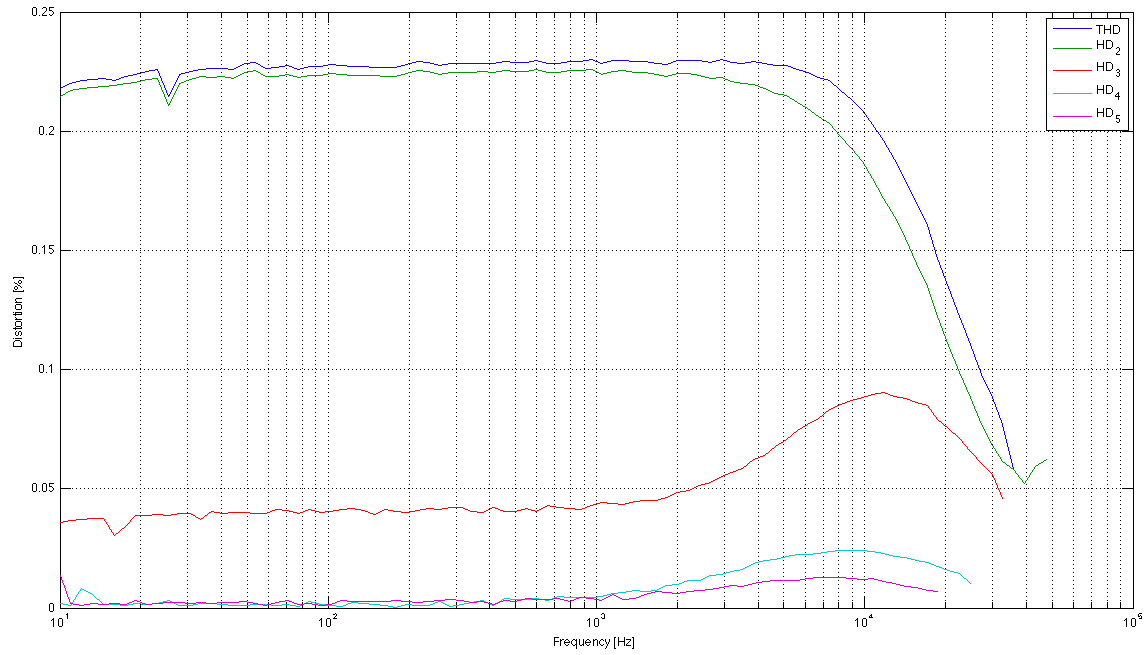
\includegraphics[width=\textwidth]{maalerapporter/forforstaerker/thd-forforstaerker.png}
\caption{Forvrængningsresultat}
\label{fig:accepttest-thdresultat-forforstaerker}
\end{figure}

\begin{figure}[h]
\centering
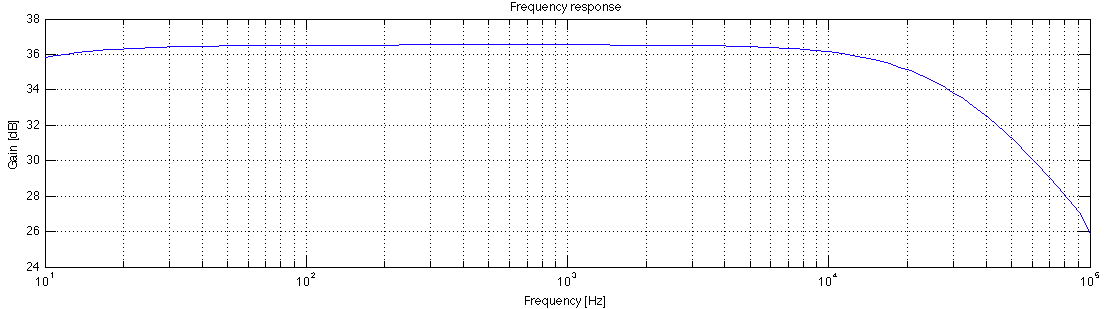
\includegraphics[width=\textwidth]{maalerapporter/forforstaerker/frekvensrespons-forforstaerker.png}
\caption{Frekvensgangs- og forstærkningsresultater}
\label{fig:accepttest-fresultat-forforstaerker}
\end{figure}

Forstærkningen ved 1 kHz er, fra resultaterne afbilledet på figur \ref{fig:accepttest-fresultat-forforstaerker}, 36,54 dB, hvilket i udregningen vist i formel (\ref{equ:accepttest-forforstaerker-db-gange}) omregnes.

\begin{equation}
\label{equ:accepttest-forforstaerker-db-gange}
10^{\frac{\mathrm{36,54~dB}}{20}} = 67,1
\end{equation}

Dette opfylder ikke kravet på 69,7 gange, men resultaterne vurderes alligevel til at være gode. Forskellen tilskrives justeringen af potentiometer under implementeringen, hvilket også vurderes til at være årsagen til forskellen i forhold til simuleringen. Frekvensgangskravene er, som det kan ses på figur \ref{fig:accepttest-fresultat-forforstaerker}, figur \ref{fig:accepttest-fres-20-63} og figur \ref{fig:accepttest-fres-125-20}, opfyldt pånær kravet ved 12,5 kHz til 20 kHz, hvor den falder 0,8 dB. Dog skulle denne blot være under 0,75 dB for at leve op til kravet, hvormed tolerancer på måleudstyret vurderes at spille ind. Derfor betragtes alle kravene som værende opfyldt.

\begin{figure}[h]
\centering
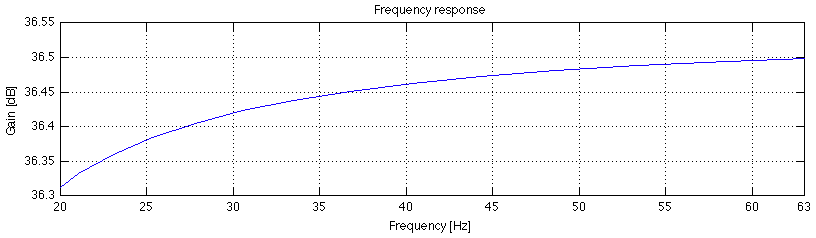
\includegraphics[width=\textwidth]{maalerapporter/forforstaerker/fr20-63.png}
\caption{Frekvensgangsresultater fra 20 Hz til 63 Hz}
\label{fig:accepttest-fres-20-63}
\end{figure}

\begin{figure}[h]
\centering
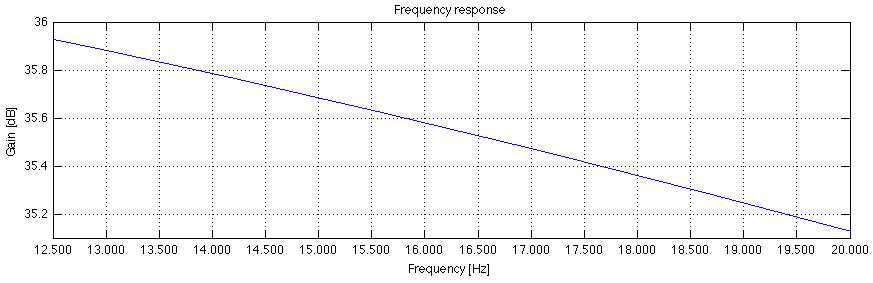
\includegraphics[width=\textwidth]{maalerapporter/forforstaerker/fr12-20k.png}
\caption{Frekvensgangsresultater fra 12,5 kHz til 20 kHz}
\label{fig:accepttest-fres-125-20}
\end{figure}